\section{Laura and the Fedeli d'Amore}

\textbf{Petrarch} wrote 300 sonnets about his love, \textbf{Laura}.

\begin{wrapfigure}{rt}{.4\textwidth}
 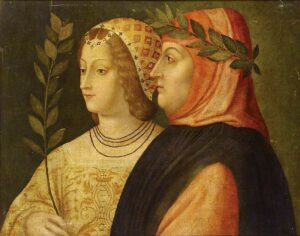
\includegraphics[scale=.45]{a20210623LauraandtheFedelidAmore-img001.jpg} 
\end{wrapfigure}

\textbf{Rene Guenon} claims that Laura was not a real woman, and that Petrarch was passing on esoteric teaching, as this quotation shows:

\begin{quotex}

The various ``ladies" celebrated by poets relating to the mysterious organization of the Fedeli d'Amore, since Dante, Guido Cavalcanti, Boccaccio and Petrarch, are not women who really lived on this earth. They are all, under different names, the one and the same symbolic ``lady", which represents the transcendent intelligence (Madonna Intelligenza de Dino Compagni) or Divine Wisdom. The most unintelligible poems in the literal sense become perfectly clear with the hypothesis of a ``jargon". In Persian Sufi writinge, a similar meaning has also been concealed under the appearances of a simple poetry of love. 

\end{quotex}
\paragraph{Sonnet \#156}
This is my translation of sonnet \#156, so you can decide if Laura is real, or perhaps it does not matter:

\begin{verse}
I saw her on earth disguised as an angel\\
Her celestial beauty was the sun in the world\\
And to remember her brings both joy and melancholy\\
As I gaze upon dreams, shadows, and smoke.

And I saw those two lovely eyes cry,\\
Which caused the sun envy again and again;\\
And I heard words said with longing\\
That would make the mountains move and rivers stand still.

Love, Wisdom, Virtue, Compassion, and Suffering\\
Make weeping a sweeter harmony\\
Than any other accustomed to be heard in the world.

Heaven was so intent on the harmony\\
That no leaf was seen to move on the bough,\\
So much sweetness had filled the air and the wind.
\end{verse}

Franz Liszt put Sonnet \#156 to music.

\url{https://www.youtube.com/watch?v=gvX5YUp9EiA}

\flrightit{Posted on 2021-06-23 by Cologero }
